\documentclass{article}
\usepackage[margin=2.5cm]{geometry}
\usepackage{parskip}
\usepackage{hyperref}

\usepackage{fontspec}
\usepackage{xltxtra}
\usepackage{amsmath}
\usepackage{graphicx}
\graphicspath{ {images/} }

% PT Serif
\setromanfont[ BoldFont=PTF75F.ttf, ItalicFont=PTZ56F.ttf,
BoldItalicFont=PTF76F.ttf, ]{PTF55F.ttf}

% Noto Sans
\setsansfont[ BoldFont=NotoSans-Bold.ttf,
ItalicFont=NotoSans-Italic.ttf, BoldItalicFont=NotoSans-BoldItalic.ttf
]{NotoSans-Regular.ttf}

\hypersetup{ colorlinks = false }


\begin{document}
\pagestyle{headings}
\textbf{\huge Software Testing Notes}\\
\textit{\footnotesize Found at: \href{http://benjaminshaw.uk}{benjaminshaw.uk}}

\section{Terms}

\textbf{Black-Box}

Examine the functionality of an application without looking at its inner workings.

\textbf{White-Box}

Testing the internal structures of an application

\textbf{ITF: Independently Testable Features}

Features that should be tested separately.

\section{Functional Testing}

\textit{\underline{Specification-based testing, black-box testing}}

A type of testing that focuses on \textit{what} the system does. Test cases are derived on the specification of the component under scrutiny.

Functional testing does not look at methods of a module, rather it tests a \textit{slice of the whole program's functionality}; verifying the program by checking it against the specification.

Functional testing is a \textit{systematic} style of testing; trying to select inputs that are \textit{valuable}.

Functional testing is \textit{not random} because its not an effective method of finding issues with the software.

\subsection{Partition Testing}

If we have knowledge that some inputs are more likely to fail than others, we can utilise this to produce more effective testing.

The entirety of possible inputs may be sparse in errors overall, but some regions may be more dense than others.

These partitions are created using the specification. These partitions will be tested, alongside their \textit{boundaries}, which tends to be an area rife with errors.

\subsection{Creating Test Cases}

\begin{enumerate}
\item
  Break the specification into \textit{Independently Testable Features}
\item 
  Identify \textit{representative} values to be used as input, \textit{e.g. correct values and malformed values}
\item
  Create \textit{test specifications} that are a combination of these inputs
\end{enumerate}

\section{Combinatorial Testing}

Where we identify some \textit{attributes} of an environment, and produce \textit{combinations} of these attributes to be tested.

\subsection{Category-Partition Testing}

Similar to functional testing, makes use of manual identification of values.

\textit{Parameters} (inputs) and \textit{environmental elements} are defined for each ITF - these values are referred to as \textit{categories}.

We generate a number of variables for each of these categories.

Finally we define constraints to remove combinations of variables that would not make sense (\textit{property constraints}), or a combination that we only need to test once, \textit{i.e. one variable renders the meaning of the other variables useless}, known as \textit{single constraints}.

The constraints allow us to reduce the number of test cases that we have, as an unwieldy test suite does not provide much benefit.

\subsection{Pairwise Combinatorial Testing}

Category partitioning is quite an exhaustive process, which pairwise combinations try to avoid.

Most bugs in software are a result of an erroneous single input. It is far less common to find a bug that involves an interaction between three or more parameters.

Pairwise covers all \underline{combinations of size 2}. This produces an inherently smaller test suite than taking the entire Cartesian product.

\subsection{Catalog Based Testing}

This method of testing is based on experience made by an organisation over time in deriving valuable test suites.

\section{Structural Testing}

\textit{\underline{Specification-based testing, glass-box testing}}

Judging test suite thoroughness based on the structure of the program itself. Structural testing is still testing product functionality against its specification. 

Specification-based testing complements and is often done after functional testing. It finds faults in parts of programs that are not executed by the functional-based testing suite. 

Structural coverage increases confidence in thoroughness of testing but \textit{\underline{it gives no guarantees }}of finding all faults, since the state might not be corrupted when statement is executed with some values.

\subsection{Statement Testing}
Statement coverage: 
$\frac{\text{\# executed statements}}{\text{\# all statements}}$

Rationale: a fault in a statement can only be
revealed by executing the faulty statement.

\subsection{Condition Testing}
Branch coverage exposes faults in how a
computation is intuitively attractive but it also groups cases with the same outcome. 

Condition coverage considers \textit{individual conditions} in a compound boolean expression.

\subsubsection{Basic condition testing}
Each basic condition must be executed at least once.

Coverage: 
$\frac{\text{\# truth values taken by all basic conditions}}{\text{2 * \# basic conditions}}$

Basic condition adequacy criterion can be
satisfied without satisfying branch coverage.

Branch and basic condition testing \textit{\underline{ are not comparable}}.

\subsubsection{Compound condition testing}

\textit{\underline{Exponential number of test cases}}

Cover all possible evaluations of compound conditions and all branches of a decision tree. 

\subsubsection{Modified condition/decision (MC/DC)}
\textit{\underline{Linear number of test cases}}. N+1 test cases for N basic conditions.

Good balance of thoroughness and test size and therefore widely used. 

Effectively test \textit{important} combinations of conditions, where \textit{important} means: each basic condition shown to independently affect the outcome of each decision. MC/DC is basic condition coverage, branch coverage with the addition of the 

Tests required:
\begin{itemize}
  \item For each basic condition C, two test cases
  \item Tests where values of all evaluated conditions except C are the same
  \item Compound condition of tests described above should evaluates to true for one value of C and false for the other
\end{itemize}

\subsection{Path testing}
Path testing focuses on combination of decisions and conditions along a path.

Path coverage: 
$\frac{\text{\# executed paths}}{\text{\# all paths}}$

Theoretically, the strongest coverage metric but generally impossible to achieve because of infeasible/infinite number of tests.

\subsubsection{Boundary interior path adequacy}
Partition the infinite set of paths into a finite number of classes. Group together paths that differ only in the subpath they follow when repeating the body of a loop. Follow each path in the control flow graph up to the first repeated node. The set of paths from the root of the tree to each leaf is the required set of subpaths for boundary/interior coverage.

\textbf{Limitations}:
\begin{itemize}
  \item The number of paths can still grow exponentially. N non-loop branches results in 2N paths.
  \item Choosing input data to force execution of one particular path may be very difficult, or even impossible if the conditions are not independent
\end{itemize}

\subsubsection{Loop boundary adequacy}
Variant of the boundary/interior criterion that treats
loop boundaries similarly but is less stringent with
respect to other differences among paths.

\textbf{Criterion}: A test suite satisfies the loop boundary adequacy criterion iff for every loop, in at least one test case, the loop body is iterated: 
\begin{itemize}
  \item zero times
  \item once
  \item more than once
\end{itemize}

\subsubsection{Linear Code Sequence And Jumps(LCSAJ) dequacy}
Often, we want to reason about the subpaths that execution can take. A subpath from one branch of control
to another is called a LCSAJ.

We can require coverage of all sequences of LCSAJs of
length N. The most basic metric is the proportion of statements executed, Test Effectiveness Ratio 1 (TER1).

TER\textsubscript{1} = Statement coverage

TER\textsubscript{2} = branch coverage

TER\textsubscript{N} = $\frac{\text{\# LCSAJ of length N executed by test data}}{\text{\# total LCSAJs of length N}}$

\subsubsection{Cyclomatic adequacy}
Cyclomatic coverage counts the number of independent paths that have been exercised, relative to the cyclomatic complexity.

Cyclomatic number - number of independent paths in the CFG. A path is representable as a bit vector, where each component of the vector represents an edge.

For e = \#edges, n = \#nodes, c = \#connected components of a graph the cyclomatic number is:

\begin{itemize}
  \item e - n + c for an arbitrary graph
  \item e - n + 2 for a CFG
\end{itemize}

\subsection{Procedure call testing}
\subsubsection{Entry and Exit Testing}
Write tests to ensure the procedure entry/exit points are entered and exited in the context they are intended to be used. Finds interface errors that statement coverage would not find.

\subsubsection{Call Coverage}
Call coverage requires that a test suite executes all possible method calls.

Challenging for OO systems, where a method call might be bound to different objects at runtime.

\subsection{Subsumption relation}
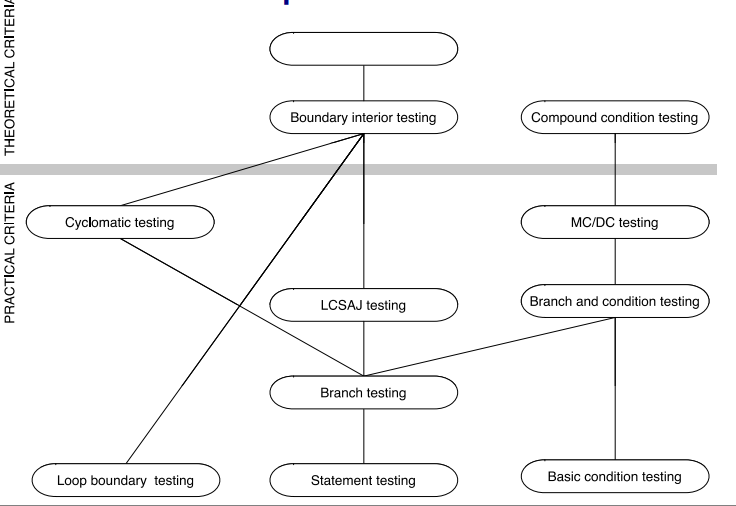
\includegraphics[scale=0.7]{subsumption_testing}

\section{Dependence and Data Flow Models}

\subsection{Def-Use Pairs}
A def-use pair associates a point in a program where a value is produced with a point where it is used.

\textbf{Definition:} where a variable gets a value
\begin{itemize}
  \item Variable declaration
  \item Variable initialization
  \item Assignment
  \item Values received by a parameter
\end{itemize}

\textbf{Use:} extraction of a value from a variable
\begin{itemize}
  \item Expressions
  \item Conditional statements
  \item Parameter passing
  \item Returns
\end{itemize}

A \textit{\underline{definition-clear path}} is a path along the CFG from a definition to a use of the same variable without another definition of the variable between.

A def-use pair is formed if and only if there is a
definition-clear path between the definition
and the use.

If, instead, another definition is present on the path, then the latter definition \textit{\underline{kills}} the former.

\subsection{Data Dependence Graph}

Nodes - same as in CFG

Edges - def-use pairs, labeled with the variable name

\subsection{Data Flow Models}
Data flow models detect patterns on CFGs:
\begin{itemize}
  \item Nodes initiating the pattern
  \item Nodes terminating it
  \item Nodes that may interrupt it
\end{itemize}

\textbf{Pros:}
\begin{itemize}
  \item Can be implemented by efficient iterative algorithms
  \item  Widely applicable (not just for classic “data flow” properties)
\end{itemize}

\textbf{Limitations:}
\begin{itemize}
  \item Unable to distinguish feasible from infeasible paths
  \item Analyses spanning whole programs (e.g., alias analysis) must trade off precision against computational cost
\end{itemize}

\section{Data Flow Testing}

Middle ground in structural testing, since node and edge coverage doesn't test interactions and path-based criteria requires impractical number of test cases.

\textbf{Criteria:}
\begin{itemize}
  \item  Each DU pair is exercised by at least one test case
  \item   Each simple(non looping) DU path is exercised by at least one test case
  \item  For each definition, there is at least one test case which exercises a DU pair containing it
\end{itemize}

\textbf{Limitations:}
\begin{itemize}
  \item  Worst case is bad (undecidable properties, exponential blowup of paths) so pragmatic compromises are required
\end{itemize}


\section{Model Based Testing}
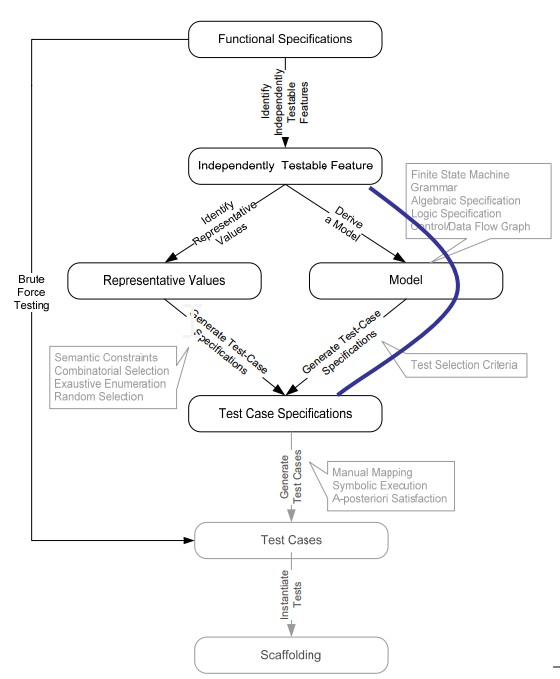
\includegraphics[scale=1.6]{model_testing}

Models are useful abstractions. In specification and design, they help us think and communicate about complex artifacts emphasizing key features and suppressing details. They convey structure and help us focus on one thing at a time.

\subsection{Deriving test cases from a FSM}
A common kind of model for describing behavior that depends on sequences of events or stimuli. E.g. UML state diagrams

\textbf{State coverage:} Every state in the model should be visited by at least one test case

\textbf{Transition coverage:} Every transition between states should be traversed by at least one test case. This is the \textit{\underline{most used criterion}}


\textbf{Base assumption:} States fully summarize history. 

So FSM testing is generally \textit{\underline{not path sensitive}} - no distinction based on how we reached a state; this should be true of well-designed state machine models. If assumption does not hold we use same criteria as in branch coverage (most commonly boundary-interior criteria).

\subsection{Deriving test cases from decision structures}
Some specifications are structured as decision tables, decision trees, or flow charts. We can exercise these as if they were program source code.


\section{Testing OOP Software}

\textbf{Characteristics of OO Software:}
\begin{itemize}
  \item State dependent behavior
  \item  Encapsulation
  \item  Inheritance
   \item Polymorphism and dynamic binding
  \item  Abstract and generic classes
  \item  Exception handling
\end{itemize}

As with testing of other software, start with functional tests and follow with structural testing.

Unit in OO is unit a class or (small) cluster of strongly related classes (e.g. sets of Java classes).

Unit testing = intraclass testing

Integration testing = interclass testing

\subsection{Intraclass Testing}

\subsubsection{State Machine Testing}
Object methods are modeled as state transitions in a FSM. Test cases are sequences of method calls.

\subsubsection{State Diagram Testing}
If state diagram is provided in the specification, use that to produce test cases. Either flatten the diagrams provided into a standard FSM or use the diagram model directly.

\subsection{Interclass Testing}

First level of integration testing for OO software. Focuses on interactions between classes.

\textbf{Approach:}
\begin{itemize}
 \item Generate class hierarchy from the class diagram. Sometimes stub generation and breaking of loops is necessary
  \item Start testing bottom-up
  \item  Consider all combinations of interactions
  \item  Select subset of these interactions(not all because of combinatorial explosion of cases). Could be random selection or significant interaction identified in the specification.
\end{itemize}

\subsection{Polymorphism and dynamic binding}
Combinatorial approach - test combination of subclasses. Same as with combinatorial testing, pairwise combinations can be used to reduce tests cases.

\subsection{Inheritance}

When testing a subclass track the overridden and newly introduced methods and only tests those.

\subsection{Exception handling}

Impractical to treat exceptions like normal flow so we separately test exceptions. We test each explicit throw or re-throw of an exception.

\vfill

\section{Mutation Testing}
\textit{\underline{Fault-based Testing:}} directed towards “typical” faults that could occur in a program.

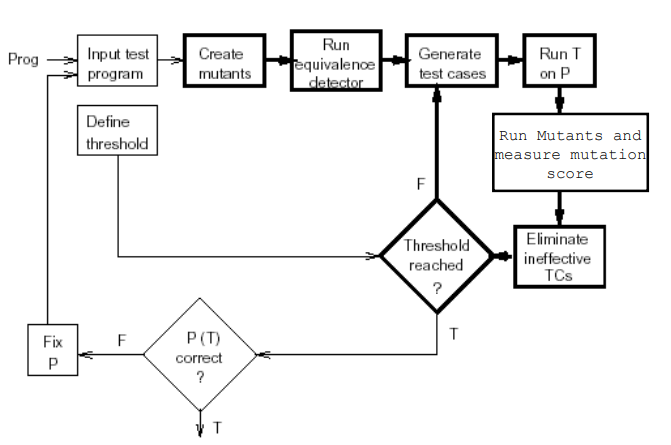
\includegraphics[scale=0.7]{mutation_testing}

\textbf{Basic idea:}
\begin{itemize}
 \item Generate class hierarchy from the class diagram. Sometimes stub generation and breaking of loops is necessary
  \item Generate test suite for a program.
  \item Create a number of similar programs by modifying the original program with small faults(mutants). This is usually done through an automated generation with specified modification rules.
  \item  Run the original test suite and ensure all faults are being caught(mutants are killed) by your tests.
    \item  If any of a mutant remains live and is not one that results in equivalent program to the original, test suite should be augmented.
\end{itemize}

\subsection{Types of mutants}

\textbf{Stillborn mutants:} Syntactically incorrect, killed by compiler, e.g., x = a ++ b

\textbf{Trivial mutants:}  Killed by almost any test case

\textbf{Equivalent mutants:} Always acts in the same behavior as the original program, e.g., x = a + b and x = a – (-b)

\textit{\underline{None of these are useful for testing}} since we want mutants that change the behavior of the program.

\section{Integration and Component-Based Testing}
Integration testing focuses on the interface specification details. It tests the interaction and compatibility between object.

Integration testing may serve as a process check for unit testing:
\begin{itemize}
 \item If module faults are revealed in integration testing, they signal inadequate unit testing .
 \item If integration faults occur in interfaces between
correctly implemented modules the errors can be correctly implemented modules, the errors can be traced to module breakdown and interface specifications. 
\end{itemize}

\subsection{Integration faults}
\begin{itemize}
 \item  Inconsistent interpretation of parameters or values. Example: Mixed units (meters/yards) in Martian Lander
 \item Violations of value domains, capacity, or size limits. Example: Buffer overflow
  \item Side effects on parameters or resources.Example: Conflict on (unspecified) temporary file
   \item  Omitted or misunderstood functionality. Example: Inconsistent interpretation of web hits
 \item Nonfunctional properties. Example: Unanticipated performance issues.
  \item Dynamic mismatches.  Example: Incompatible polymorphic method calls
\end{itemize}

\subsection{Big Bang Integration Testing}
Test only after integrating all modules. Does not require scaffolding  but has a lot of drawbacks: high cost of repair, minimum observability, diagnosability, efficacy and feedback.

\subsection{Structural orientation}
Modules constructed, integrated and tested based on a hierarchical project structure.

\subsubsection{Top down}
Working from the top level (in terms of “use” or “include” relation) toward the bottom. No drivers required if program tested from top-level interface (e.g. GUI, CLI, web app, etc.). Write stubs of called or used modules at each step in construction. As modules replace stubs, more functionality is testable.

\subsubsection{Bottom up}
Starting at the leaves of the hierarchy, we never need stubs but we must construct drivers for each module. When an intermediate module replaces a driver, it needs its own driver. Several working subsystems, consisting of method and drivers, eventually get integrated into a single system.

\subsubsection{Sandwich}
Start testing from both ends. Both stubs and drivers needed. Sandwich integration is flexible and adaptable but complex to plan.

\subsection{Functional orientation}
Modules integrated according to application characteristics or features. Functional strategies require more planning and are more complex than structural strategies but provide better process visibility, especially in complex systems.

\subsubsection{Threads}
A “thread” is a portion of several modules that together provide a user-visible program feature. Integration is done one thread at a time. Minimizes stubs and drivers but is also complex to plan.

\subsubsection{Critical Modules}
Start integration form riskiest modules. Risk assessment is necessary first step. Designed to deliver any bad news as early as possible.

\subsection{Component Testing}

Components are reusable units of deployment and composition. They are often deployed and integrated multiple times and are characterized by an interface or contract. Usually integrated and tested by different teams. 

\subsubsection{Producer View Testing}
Includes thorough functional testing based on application program interface (API). Includes thorough acceptance testing based on scenarios of expected use. Includes stress and capacity testing.

\subsubsection{User View Testing}
Not primarily to find faults in the component. More concerned with the question of if the component is suitable for this application.

\section{Test Driven Development}
Only relevant to black-box unit testing.

\subsection{TDD cycle}
\begin{itemize}
\item \textbf{Write Test Code:} Guarantees that every functional code is testable. Provides a specification for the functional code.Helps to think about design.Ensure the functional code is tangible
\item \textbf{Write Functional Code:}  Fulfill the requirement (test code). Write the simplest solution that works. Leave Improvements for a later step. The code written is only designed to pass the test

\item \textbf{Refactor:} Clean-up the code (test and functional). Make sure the code expresses intent. Remove code smells. Re-think and design. Delete unnecessary code.
\end{itemize}


\subsection{Advantages}
\begin{itemize}
 \item  Shortens the programming feedback loop.
  \item Promotes the development of high-quality
code
  \item User requirements more easily understood.
  \item  Reduced interface misunderstandings
   \item   Provides concrete evidence that your
software works
\item Reduced software defect rates, better code and less debug time
\end{itemize}

\subsection{Disadvantages}
\begin{itemize}
 \item  Programmers like to code, not to test
  \item Test writing is time consuming
  \item  Test completeness is difficult to judge
\end{itemize}

\section{Regression Testing}

Changes in software that introduce software bugs and make features stop functioning as intended are called \textit{\underline{regressions}}. To avoid regressions old test should be run in addition to tests added for new additions in the software.

\subsection{Re-test All}
The test-all approach is good when you want
to be certain that the new version works on all
tests developed for the previous version. Becomes increasingly expensive as software grows. Bad if you have limited resources.

\subsection{Re-test Test Suite Subset}

\subsubsection{Code-based selection}
Only execute test cases that execute changed or new code.

\subsubsection{Control-flow and data-flow selection}
Same idea as code-based selection but it analyses changes in the control-flow and data-flow graphs. Can be automated.

\subsubsection{Specification-based  selection}
Pick test cases that test new and changed
functionality.

\subsection{Program Dependence Graph}

Program Dependence Graph (PDG) that captures control and data dependencies between nodes in CFG.

Automated analysis can be done against the PDG to prioritize tests to be run.

\section{System \& Acceptance Testing}
\subsection{System Testing}
Tests for correctness and completion.

One strategy for maximizing independence:
System (and acceptance) test performed by a different organization than the one doing the implementation.

Major focus of system testing is the opportunity to verify global properties against actual system specification. Global properties - performance, latency, reliability. Those properties can vary depending on the testing environment.


\subsubsection{Stress testing}
\subsubsection{Capacity testing}
\subsubsection{Security testing}
\subsubsection{Performance testing}
\subsubsection{Compliance testing}
\subsubsection{Documentation testing}

\subsection{Acceptance Testing}
Used to measure quality quantitatively.
\subsubsection{System Reliability}
\subsubsection{Component Reliability Model}
\subsubsection{MTTF: Mean Time To Failure}
\subsubsection{Serial System Reliability}
\subsubsection{Parallel System Reliability}

\end{document}